\graphicspath{{RL/fig}}
\chapter{Dynamic Programming and Reinforcement Learning}
\label{chap:RL}

\section{Introduction}
This chapter can be divided into three sections. Dynamic programming which \textbf{solves} a \textit{\textbf{known}} MDP, model-free prediction which \textbf{estimates} an \textit{\textbf{unknown}} MDP and model-free control which \textbf{optimizes} the value function of an \textit{\textbf{unknown}} MDP.

\section{Dynamic Programming}
\subsection{Background}
Dynamic programming is a method to solve problems by using a divide and conquer approach. That is to say a problem is broken into smaller sub-problems and then solved.
There are two properties that must be met for a problem to be solvable via Dynamic Programming: Optimal substructure and Overlapping sub-problems. \cite{David_Silver}
\begin{itemize}
	\item Optimal substructure requires that the solution be able to be decomposed into sub-problems.
	\item Overlapping sub-problems requires that the sub-problems occur many times over, meaning that the solution can be cached and reused.
\end{itemize}

Markov decision processes satisfies both of these conditions. The Bellman equation provides a recursive decomposition which fulfills the Optimal substructure property. While the value function caches and reuses solutions satisfying the Overlapping sub-problems condition. \cite{David_Silver}\\

\subsection{Iterative Policy Evaluation}
In order to evaluate the value that a certain policy has, we use a method called \textit{Iterative Policy Evaluation}. Figure \ref{fig:iterative_policy_evaluation} shows the mathematics which describes Iterative Policy Evaluation in both summation and vector form. What the diagram  at the top of Figure \ref{fig:iterative_policy_evaluation} represents is the value function being calculated for an action 'a' to an intermediary state represented by the black dot. The environments reaction is then also accounted for from the intermediary state to state s' resulting in reward r. The environments information is contained in the transition probability matrix $P^\pi$.

We then use state s' as the new start state s and repeat the same calculation.
The value function is updated continuously until the difference between $v^{k}$ and $v^{k+1}$ is determined negligible.

\begin{figure}
	\centering
	\begin{subfigure}{.49\textwidth}
		\centering
		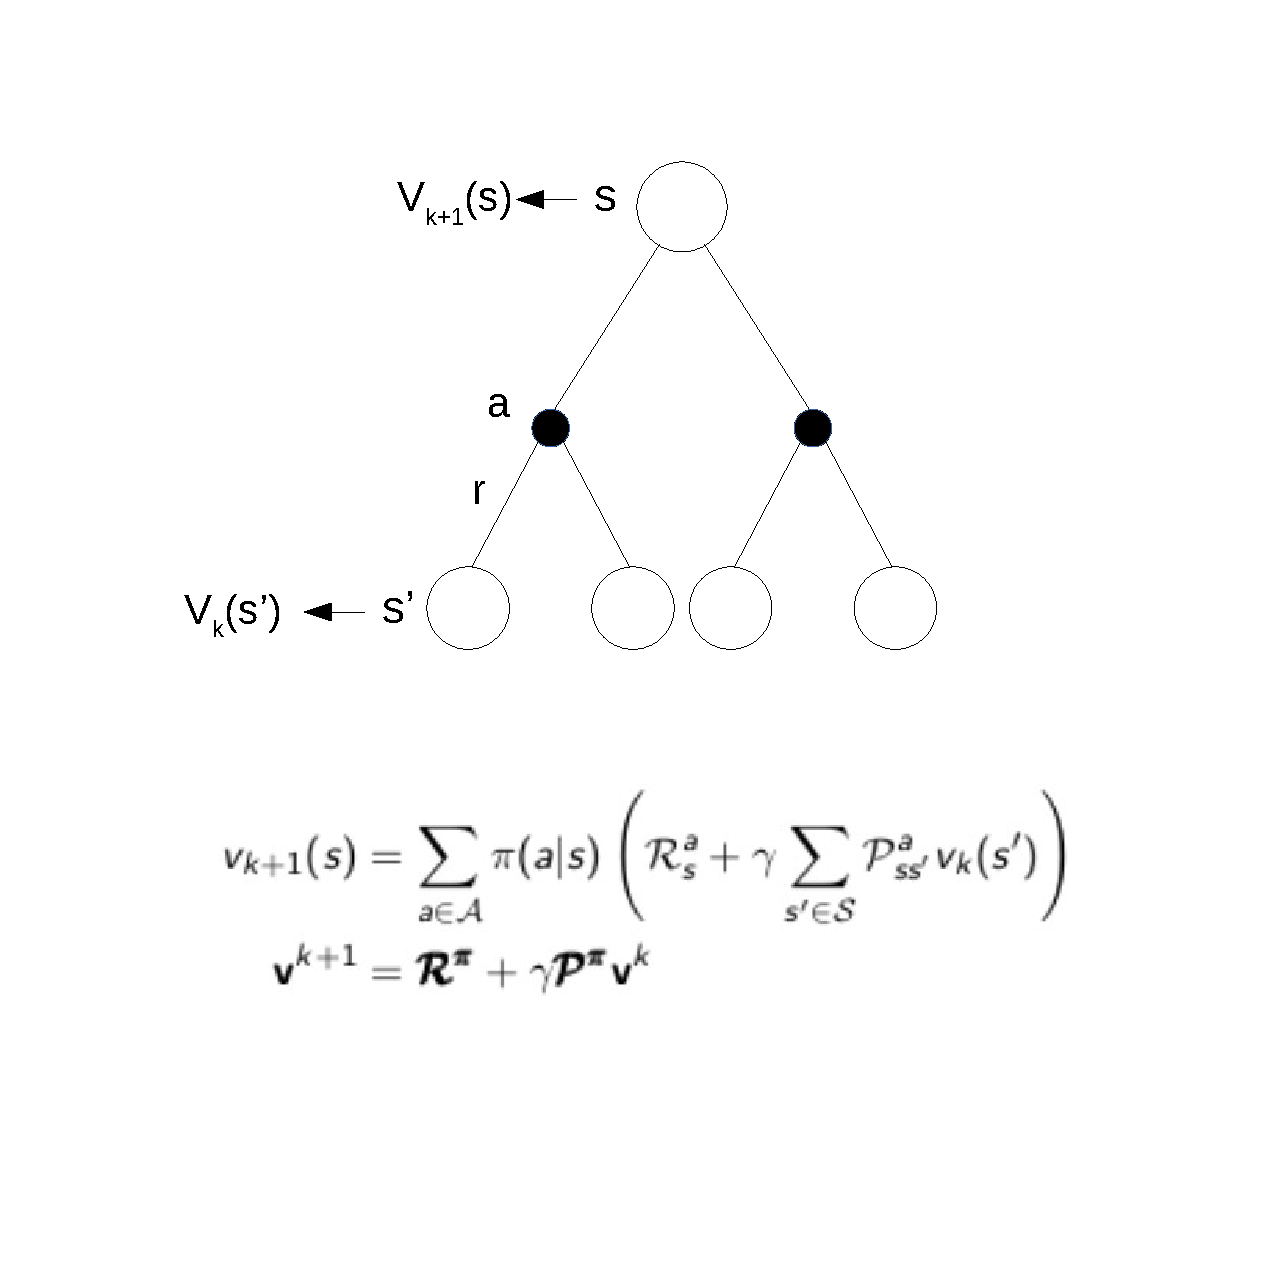
\includegraphics[width=1\linewidth]{MDP/fig/Iterative_Policy_Evaluation.png}
		\caption{Iterative policy Evaluation\cite{David_Silver}}
		\label{fig:iterative_policy_evaluation}
	\end{subfigure}
	\begin{subfigure}{.49\textwidth}
		\centering
		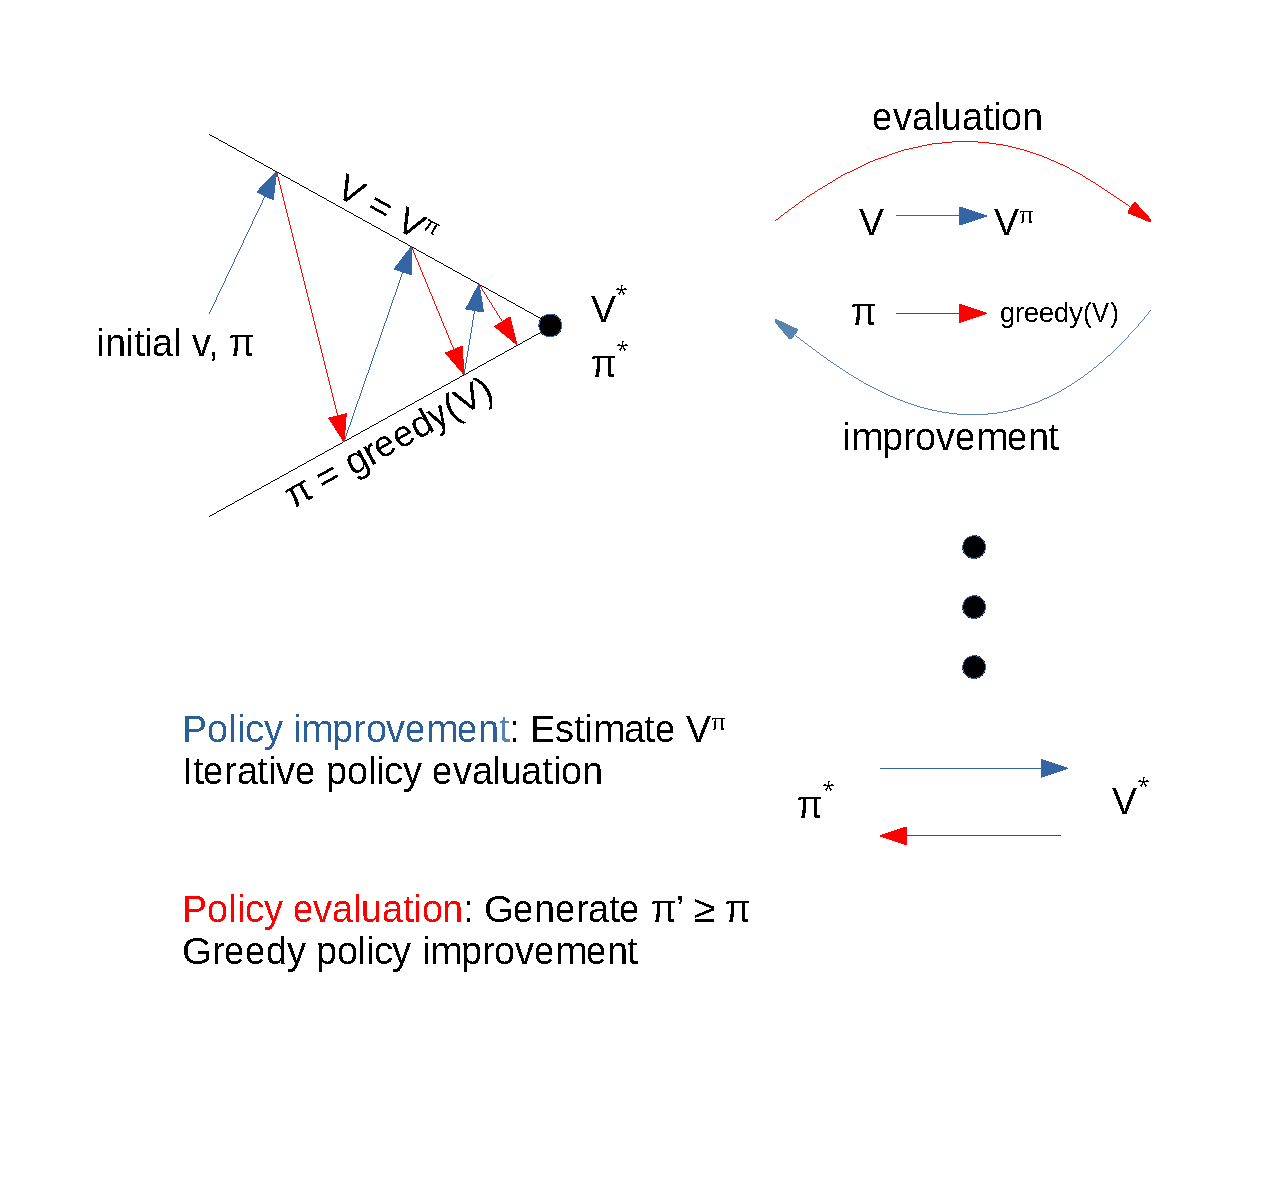
\includegraphics[width=1\linewidth]{MDP/fig/Policy_iteration.png}
		\caption{Greedy Policy iteration visualisation\cite{David_Silver}}
		\label{fig:greedy_policy_iteration}
	\end{subfigure}
	\caption{Policy Iteration \cite{David_Silver}}
	\label{fig:policy_iteration}
\end{figure}

\subsection{Policy Iteration}
There are two separate uses for Dynamic Programming in Reinforcement Learning. These are prediction and control which both have $(S,A,P,R,\gamma)$ as input.
\begin{itemize}
	\item The prediction method uses $(S,A,P,R,\gamma)$ and a policy $\pi$ as input, while it outputs a value function $v_\pi$.
	\item The control method only takes $(S,A,P,R,\gamma)$ as input and outputs the optimal value function $v_*$ and optimal policy $\pi_{*}$.
\end{itemize}
{\color{red} Maybe insert a flow diagram illustrating difference and similarity between prediction and control }

These two methods of Dynamic programming are implemented via what is known as value iteration and policy iteration respectively.
Figure \ref{fig:greedy_policy_iteration} shows how Greedy Policy Iteration works. A greedy policy is one which when followed, results in the maximum value function $v_\pi$. It is known that policy iteration converges which can also be seen in the diagram in Figure \ref{fig:greedy_policy_iteration} on the top left.\cite{sutton_barto}

As is stated in Figure \ref{fig:greedy_policy_iteration} policy iteration works by continuously iterating between two steps, namely policy evaluation and policy improvement.


For a given policy $\pi$ we improve the policy using the following two steps:\\\\
\textbf{Step one} is \textit{Evaluating} the policy $\pi$ using equation \ref{bellmanv2}: \[v_{\pi}(s) = E_{\pi}[R_{t+1} + \gamma v_{\pi}(S_{t+1})|S_t = s]\]
\textbf{Step two} is \textit{Improving} the policy by acting greedy with respect to $v_\pi$ to obtain a new policy $\pi^{'}$:
\begin{align}
	\pi^{'} &= greedy(v_{\pi})= v_{*}
	\label{pi'}
\end{align}
\[\pi^{'}(s) = \max\limits_{a}(R^{a}_s+\gamma\sum_{s'\in S}P^{a}_{ss'}v_*(s'))\]

What this means is that we obtain a value function by using iterative policy evaluation where after we update the policy. In this way we will always converge to the optimal policy $\pi_{*}$ and value function $v_{*}$ described by equation \ref{eq:pi_*} and \ref{bellmanv*} respectively.
\subsection{Value Iteration}
\begin{figure}[!htb]
	\centering
	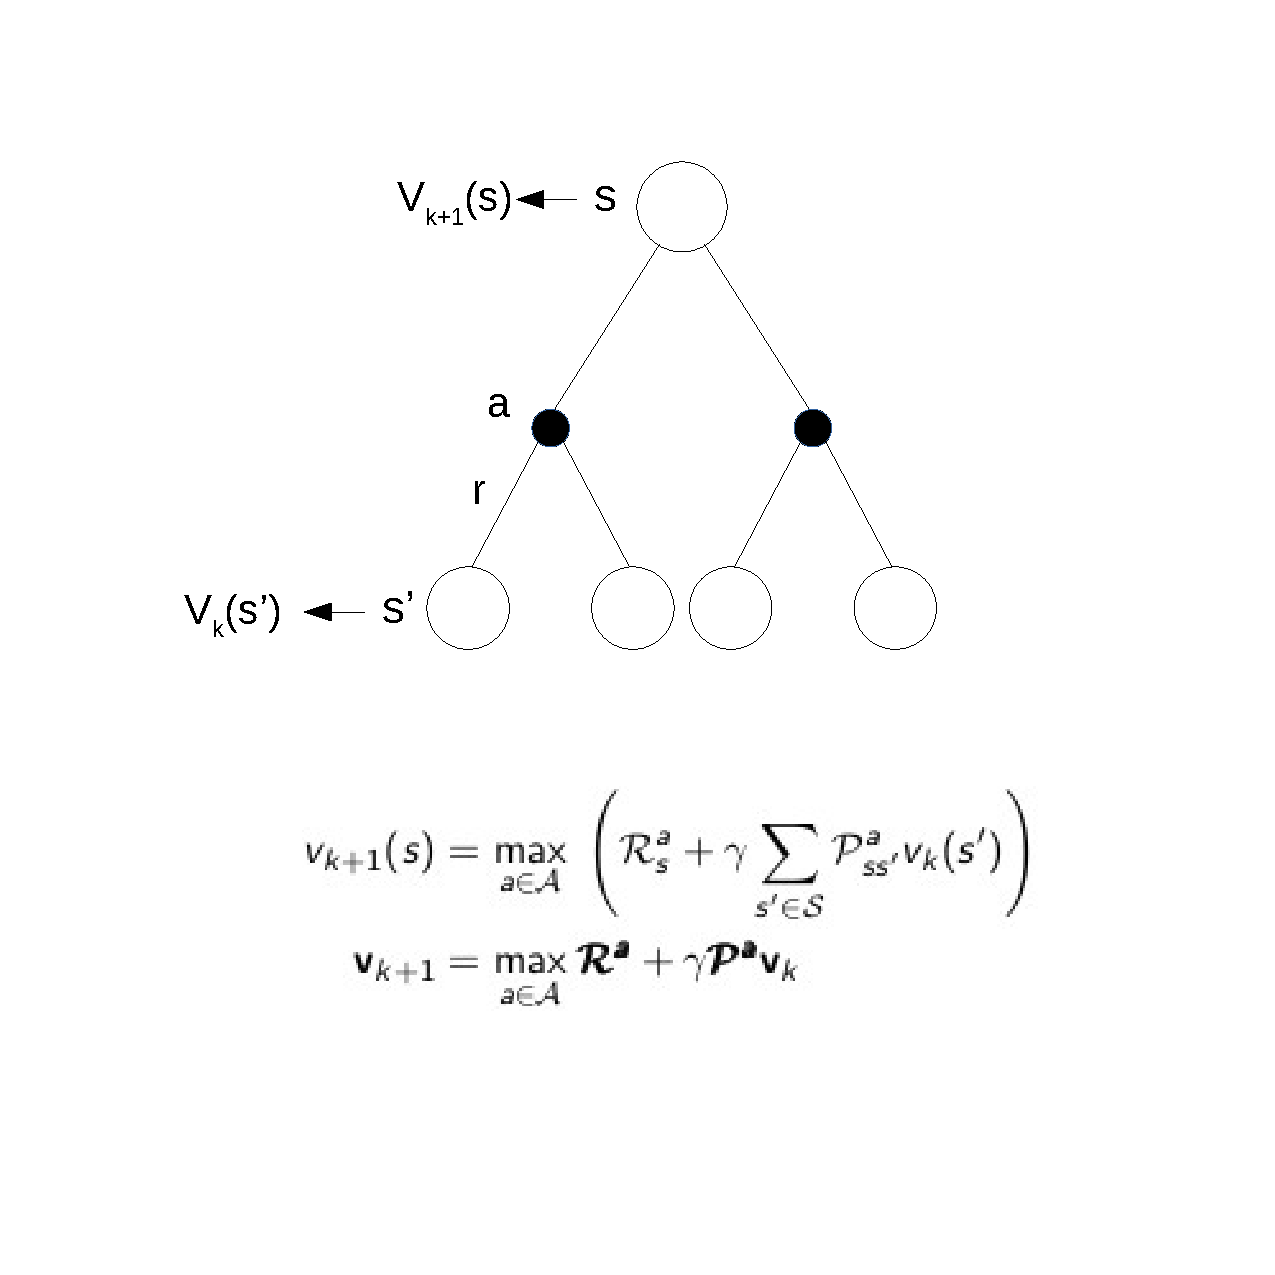
\includegraphics[width=0.75\linewidth]{MDP/fig/value_iteration.png}
	\caption{Value Iteration\cite{David_Silver}}
	\label{fig:value_iteration}
\end{figure}
Figure \ref{fig:value_iteration} shows the mathematics that describes \textit{Value Iteration}. It is very similar to iterative policy evaluation in Figure \ref{fig:iterative_policy_evaluation}. Iterative Policy Evaluation calculates the value function for a policy $\pi$ which is an entire set of actions given states.

While Value Iteration calculates the maximum value function for a single action only. In this sense Value Iteration is a special case of Iterative Policy Evaluation.

{\color{red} Can later place in appendix proof of policy iteration always converging. slide 19 (16/42) of David Silvers slides on Dynamic Programming}
\section{Reinforcement Learning}
What we have been discussing up to now all has had to do with using methods which required knowledge about the model. This knowledge was embedded in the probability transition matrix P. Often times this matrix P is extremely large making calculation times long. While at other times it is not possible to know the model of the environment beforehand. We therefore look at methods which do not need models.

There exists both model-free prediction and model-free control Reinforcement Learning techniques.
Model-free \textbf{prediction \textit{evaluates}} the value function of an unknown MDP.
While Model-free \textbf{control \textit{optimizes}} the value function of an unknown MDP.

There are two ways that model-free control can be implemented:

\textbf{On-policy learning:}
Learning characteristics of a policy $\pi$ by sampling from $\pi$

\textbf{Off-policy learning:}
Learn characteristics of policy $\pi$ by sampling another policy $\mu$

\subsection{Model-free prediction}
\subsubsection{Monte-Carlo Policy evaluation}
Monte-Carlo policy evaluation works as follows:
When time step t and state s is reached we increment a running counter N(s) = N(s)+1. This can be done in two ways, one being only incrementing N(s) the \textit{first} time state s is reached or incrementing N(s) \textit{every} time states s is reached.

Then we increment the total reward to S(s) =  S(s) + $G_t$.

Finally we calculate the value function $V(s)=\frac{S(s)}{N(s)}$

Then V(s) $\to V_\pi(s)$ as N(s) $\to \infty$

In order to incrementally do Monte-Carlo updates,an incremental mean $u_k$ is used. The derivation for $u_k$ from a standard mean is as follows:
\begin{align}
	u_k &= \frac{1}{k}\sum_{j=1}^{k}x_j\\
	&= \frac{1}{k}(x_k + \sum_{j=1}^{k-1}x_j)\\
	&= \frac{1}{k}(x_k +(k-1)u_{k-1})\\
	&= u_{k-1} + \frac{1}{k}(x_k - u_{k-1})
	\label{eq:u_k}
\end{align}
The variable that we are averaging over is V(s) hence $V(s)=u_{k-1}$ and the counter $N(s)=k$ in equation \ref{eq:u_k}. The return $G_t =x_k$. Hence at every time t:

\begin{align}
	N(S_t) &= N(S_t) + 1 \\
	V(S_t) &= V(S_t) + \frac{1}{N(S_t)}(G_t - V(S_t))
\end{align}
It can be useful to forget old states by making $N(S_t)$ a constant $\alpha$ as follows:
\begin{equation}
	V(S_t) = V(S_t) + \alpha(G_t - V(S_t))
	\label{eq:monte_carlo}
\end{equation}


\subsubsection{Temporal Difference (TD) Learning}
Temporal difference (TD) learning is a technique used to predict the value of a signals future state.

The aim of TD learning is to learn a value function $v_\pi$ from experience of following policy $\pi$. 
The simplest form of TD is replacing the return $G_t$ in equation \ref{eq:monte_carlo} as follows:
\begin{equation}
	V(S_t) = V(S_t) + \alpha({\color{red}R_{t+1} +  \gamma V(S_{t+1})} - V(S_t))
	\label{eq:monte_carlo_TD}
\end{equation}
${\color{red}R_{t+1} +  \gamma V(S_{t+1})}$ is known as the TD target, the value which $V(S_t)$ tends to as $t \to \infty$.
${\color{red}R_{t+1} +  \gamma V(S_{t+1})} - V(S_t)$ is known as the TD error. The aim of TD is to reduce the TD error to zero and update $V(S_t)$ to the estimated return ${\color{red}R_{t+1} +  \gamma V(S_{t+1})}$.
\begin{figure}[!htb]
	\centering
	\begin{subfigure}{.5\textwidth}
		\centering
		\includegraphics[width=0.5\linewidth]{RL/fig/mc_backup.png}
		\caption{Monte Carlo backup\cite{David_Silver}}
		\label{fig:monte_carlo_backup}
	\end{subfigure}
	\begin{subfigure}{.49\textwidth}
	\centering
	\includegraphics[width=0.5\linewidth]{RL/fig/mctd_backup.png}
	\caption{Temporal difference backup\cite{David_Silver}}
	\label{fig:monte_carlo_TD_backup}
	\end{subfigure}
	\caption{MC and TD visual representations using n-return \cite{David_Silver}}
	\label{fig:MC_TD_backups}
\end{figure}

\begin{figure}[!htb]

\end{figure}
Figure \ref{fig:monte_carlo_backup} and \ref{fig:monte_carlo_TD_backup} shows the concepts of MC and TD learning visually presented. Mathematically we can show the relationship between MC and TD using the n-step return concept, which will now be described.

Let the n-step return be defined as:
\begin{equation}
	G_{t}^{(n)} = R_{t+1} + \gamma R_{t+2} + ... + \gamma^{n-1}R_{t+n} + \gamma^{n}V(S_{t+1})
\end{equation}
For clarity we show 
$G_{t}^{(n)}$ for a few values of n as follows:\\
\begin{align}
	 {\color{red}(TD)} n &= 1: G_{t}^{(1)} = R_{t+1}+\gamma V(S_{t+1}) \label{eq:td} \\
	n &= 2 : G_{t}^{(2)} = R_{t+1}+ \gamma R_{t+2}+\gamma^2 V(S_{t+2}) \\
	{\color{red}(MC)} n &= \infty : G_{t}^{(\infty)} = R_{t+1}+ \gamma R_{t+2}+...+\gamma^{T-1} R_T \label{eq:mc_td}
\end{align}
Figure \ref{fig:monte_carlo_backup} corresponds to equation \ref{eq:monte_carlo} and \ref{eq:td}. While Figure \ref{fig:monte_carlo_TD_backup} to equation \ref{eq:monte_carlo_TD} and \ref{eq:mc_td}. We now define n-step TD as:
\begin{equation}
	V(S_t) = V(S_t) + \alpha(G_t^{(n)} - V(S_t))
	\label{eq:n_step_TD}
\end{equation} 
What we now have is a function with which we can choose when to update V(S), instead of always having it update at the end of the episode like MC. This is useful because we can correct mistakes made in the prediction earlier if n-step TD is used.
\subsection{Model-free control}

When we previously used greedy policy improvement over the value function V(s) we had in equation \ref{pi'}:
\[\pi^{'}(s) = \max\limits_{a \in A}(R^{a}_s+\gamma\sum_{s'\in S}P^{a}_{ss'}v_*(s'))\]
Now for greedy policy improvement over the state action function Q(s,a) we have that:
\begin{equation}
	\pi^{'}(s) = \max\limits_{a \in A}Q(s,a)
\end{equation}
Which means that we now maximize not only across the action set as in equation \ref{pi'}, but rather the entire state-action set when using model-free policy iteration.

However there now arises a problem when always having the agent act greedily. Which is that the agent will always take the same path no matter whether another path might have been better in the long term. To overcome this limitation of we bring in the topic of $\epsilon$-Greedy exploration.

To ensure that the agent explores occasionally instead of always taking the greedy action, let the agent act randomly with a probability $\epsilon$. This can mathematically be expressed as:
\begin{align}
	\pi(a|s)=\begin{cases}
		\frac{\epsilon}{m}+1, & \text{if $a^* = \argmax\limits_{a \in A}Q (s,a)$}\\
		\frac{\epsilon}{m}, & \text{otherwise}
	\end{cases}
	\label{eq:pi_epsilon-greedy}
\end{align}
One can note that equation \ref{eq:pi_epsilon-greedy} is a variation of equation \ref{eq:pi_*}.

\subsubsection{SARSA}

\subsubsection{Q-learning}